\documentclass{acmsiggraph}

\usepackage{parskip}
\usepackage{graphicx}
\usepackage{courier}
\usepackage{footmisc}
\usepackage{listings}
\usepackage{amsmath}
\usepackage{url}
\usepackage{color}
\usepackage{xcolor}
\onlineid{0}

\title{Cinematic Particle Systems with OpenCL}

\author{Tim Horton\thanks{e-mail: hortot2@rpi.edu}\\Rensselaer Polytechnic Institute}

\begin{document}

\maketitle

\begin{figure}
    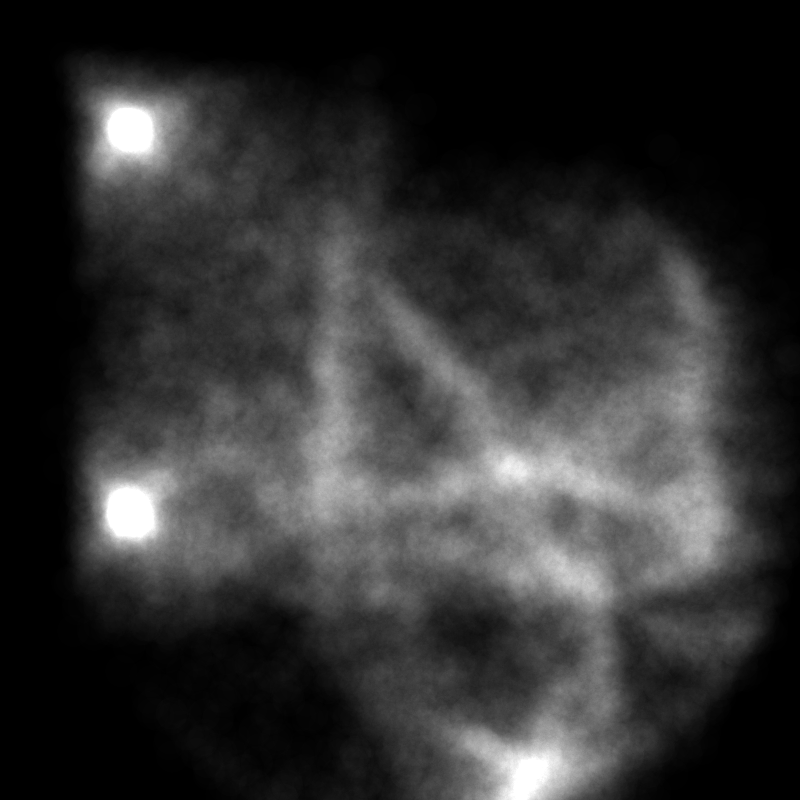
\includegraphics[width=84.5mm]{gravity.png}
    \caption{A simple gravity simulation with two emitters and three supermassive particles (approx. 45,000 particles)}
\end{figure}

\section*{Abstract}

High-particle-count simulations are becoming increasingly crucial in many different aspects of our world today: both in entertainment --- within video games, movies, and the like --- and in scientific fields, where particle systems are capable of simulating and visualizing many interesting phenomena.

This paper will explore the possibility of parallelizing the simulation of these large particle systems and offloading them to very-parallel\footnote{As opposed to {\it massively-}parallel, like the CCNI's Blue Gene/L, or the {\it slightly}-parallel CPU in most modern computers} hardware which is usually only used for {\it rendering}: the video card.

We will also touch briefly on ways to design a system for describing particle systems in a generalized way, though the majority of the work that is currently in a functional state centers around simulation and rendering.

\section{Introduction}

Simulation of large particle systems requires a large amount of computation --- each particle must be inspected and updated. For certain types of particle systems --- n-body gravity, for example --- each particle is affected by its neighbors, increasing the required calculation time drastically.

This is what we aim to address with this paper. While it's unlikely that we can contribute any improved simulation algorithms, we can instead work to parallelize these algorithms and implement them with OpenCL, which will allow them to run on the GPU contained within modern graphics cards. This paper will demonstrate both the parallelization of the application of forces on large numbers of particles and the significant performance gained by doing so.

We will also explore a simple parallelized particle renderer, as well as the potential for the integration of our simulator into the popular open-source 3D package, Blender.

It is important to understand that the system we've developed is purely for offline work --- it is not suitable for realtime simulation and rendering. Thus, {\it cinematic}. This is primarily because of the relatively poor performance of the renderer. However, as you'll notice in section \ref{performanceSection}, the speedup provided by our work {\it is} actually sufficient to make some simulations fast enough to run in real time, if one were to find a faster renderer.

\section{Prior Art}

\section{Implementation}

The code for this paper is available under the 2-clause BSD license at:

\url{http://github.com/hortont424/particles}

It consists of about 3000 lines\footnote{According to {\it sloccount}} of C and Objective C, which encompass the curve editor and other design tools, an abstraction layer on top of OpenCL\footnote{the Open Computing Language, a framework for creating programs using a language similar to GLSL and run on the GPU}, and all of the code to drive simulation, preview, and rendering. In addition, there are about 350 {\bf [UPDATE THIS]} lines of OpenCL Kernel Language, which includes the code to apply each of the forces as well as the renderer.

\subsection{Particle Systems}

A particle system is defined by a simple JSON\footnote{JavaScript Object Notation, a format often used today for information exchange in place of things like XML, due to its lightweight nature} file (figure \ref{curveListing} is a very simple example of such a file), which lays out all of the system's parameters: the number of particles to start out with, the location and properties of emitters, the location and properties of forces, and many other things. If {\it Interpolator} had been finished, this file would also contain the mappings between these properties and various curve files.

\begin{figure}

    \lstset{language=Python}
    \lstset{basicstyle=\footnotesize\ttfamily}
    \lstset{stringstyle=\color{blue}\ttfamily}
    \begin{lstlisting}[frame=trbl]{}
{
    "initialParticles": {
        "count": 1
    },
    "forces": [
        {
            "kernel": "gravity",
            "strength": 1.0,
            "noise": 0.0,
            "mass": 100000000000.0,
            "particle": {
                "fixed": true,
                "x": 1.2,
                "y": 1.2,
                "z": 0.5
            }
        }
    ],
    "emitters": [
    {
        "birthRate": 20.0,
        "initialVelocity": 0.0,
        "particle": {
            "fixed": true,
            "x": -1.2,
            "y": 1.2,
            "z": 1.5
        }
    }],
    "integration": {
        "kernel": "verlet",
        "timestep": 0.005
    }
}
    \end{lstlisting}

    \caption{A simple sample curve file, with one emitter and one force}
    \label{curveListing}
\end{figure}

\subsection{Design}

\begin{figure}
    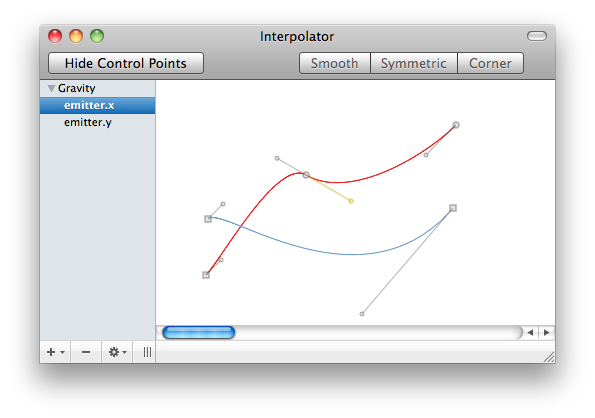
\includegraphics[width=84.5mm]{interpolator.png}
    \caption{A screenshot of the unfinished {\it Interpolator} particle system design tool}
    \label{fig:interpolator}
\end{figure}

The particle system design tools implemented during the course of this project are not entirely functional, as they took a backseat to the simulation, preview, and rendering components, mostly due to the fact that it's possible to design a system by hand.

The primary design tool, which can be seen in figure \ref{fig:interpolator}, is called {\it Interpolator}, as it is quite literally a tool to design interpolation curves. It's a Cocoa application which provides an interface to edit arbitrary B\'{e}zier splines and map them to properties of an element in the particle system. For example, one curve might dictate the $x$ position of an emitter, while another might be mapped to the lifetime that emitter's children.

\subsection{Simulation}

\subsubsection{Physics}

\subsection{Preview}

\begin{figure}
    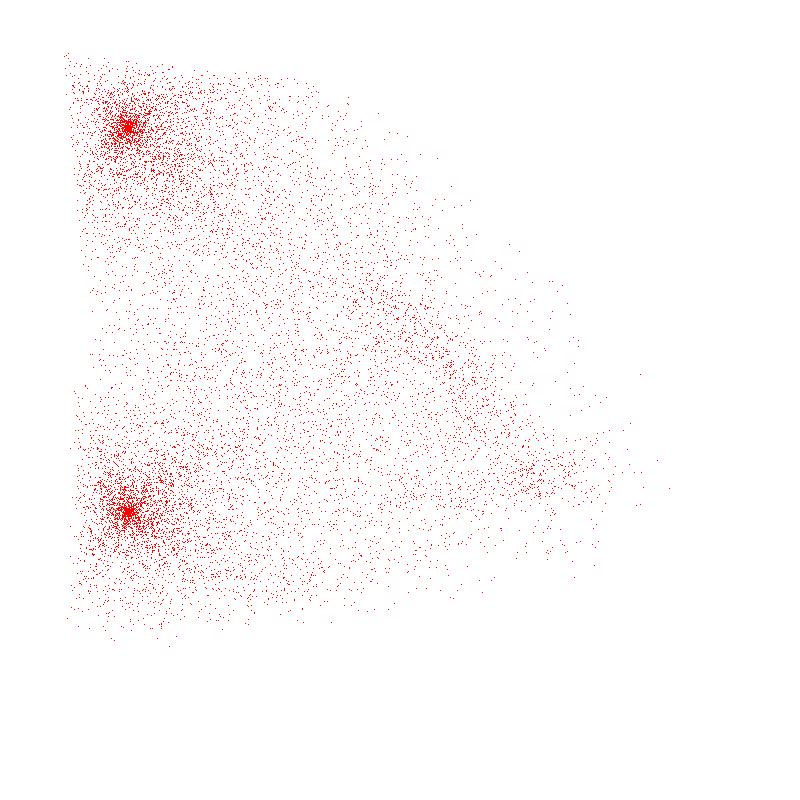
\includegraphics[width=84.5mm]{preview.png}
    \caption{Example frame of preview output (simple gravity system); approximately 15,000 particles}
    \label{fig:preview}
\end{figure}

\subsection{Rendering}

\section{Performance \& Results}

\label{performanceSection}

\begin{figure}
    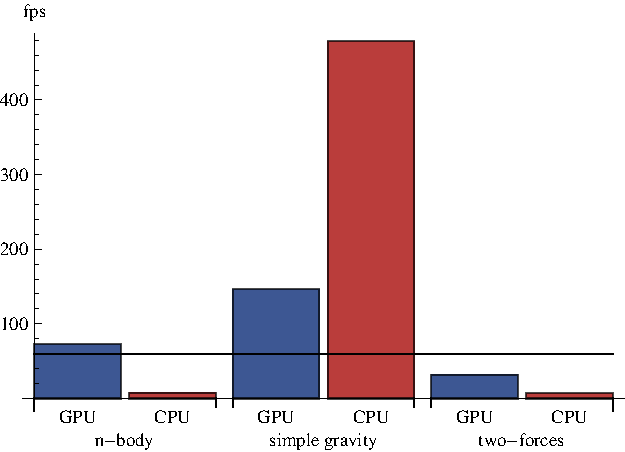
\includegraphics[width=84.5mm]{basicSpeedPlot.pdf}
    \caption{Simulation frame-rate of various different systems on CPU vs. GPU; higher values are better; the horizontal line rests at 60 fps}
    \label{fig:basicSpeedPlot}
\end{figure}

\subsection{Hardware}

\subsection{Benchmarks}

\subsection{Video}

\section{Applications}

\section{Future Work}

\subsection{Spatial Hashing}

One improvement which would massively improve the performance of both the renderer and some of the forces would be the inclusion of a spatial hashing mechanism.

For example, the renderer currently iterates over all of the particles to find the few which are very close to the pixel currently being rendered --- this operation is currently implemented in the most na\"{i}ve way possible, which is $O(n^2)$. The implementation of a kd-tree would make this $O(n^{2/3})$ instead --- quite a significant improvement, though at the expense of a measurable increase in complexity.

\subsection{Design Tools}

\subsection{Extended Properties}

\subsection{Rendering Improvements}

\subsection{Blender Integration}

\section{Conclusion}

\bibliographystyle{acmsiggraph}
\nocite{*}
\bibliography{report}

\end{document}